\section{V8}
\begin{minipage}[t]{9cm}
	\subsection{Cortex M3 Instruction Set}
	\subsubsection{Thumb-2 Instruction Set}
    \begin{tabular}{l l}
        Ziel:&-Erhöht die Code-Dichte\\
            &  -Mehr Leistung\\ 
        Cortex M3 Processor:  & 1.25 DMIPS / MHz\\ 
    \end{tabular} 
    
\subsection{Instruction Pipelining}
                  Mit Pipelining bearbeitet der Cortex-M Prozessor zur gleichen Zeit drei Befehle - jeweils um einen Takt versetzt.\\
     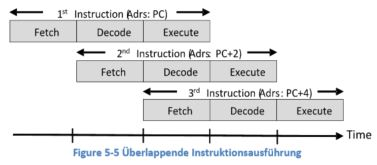
\includegraphics[width=9cm]{images/pipelining}\\
     \begin{tabular}{m{1.5cm} m{6.5cm}}
        Fetch:& 16-Bit Instruktion aus Programmspeicher laden\\
        Decode:& Vorangehende Instruktion decodieren\\ 
        Execute:& Nochmals vorangehende Instruktion ausf"uhren\\
    \end{tabular} 
    Bei einem Sprung im Programmcode muss eine Pipeline komplett geleert werden, da die sequentielle Reihenfolge je nach Konstellation nicht korrekt ist.
\end{minipage}
%
\begin{minipage}[t]{0.5cm}
	\-\
\end{minipage}
%
\begin{minipage}[t]{9cm}
	\subsection{Logikstruktur des Cortex-M Prozessor}
        \begin{tabular}{ll} 
            Sourceoperanden:& Rn, Rm \\ 
            Destinationsoperand:& Rd  \\ 
            MAC:& Memory Access Calculator\\

        \end{tabular} \\
        Ein \textit{Barrel-Shifter} vereinfacht Berechnungen,\newline
        da Multiplikationen einfacher realisiert werden können.\\
        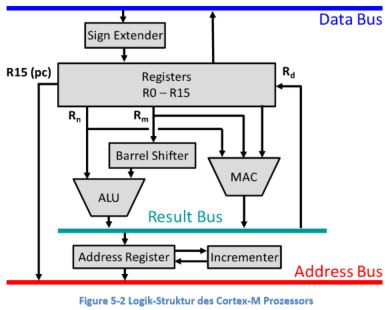
\includegraphics[width=9cm]{images/logikstrukturcortex}
        
        Das 32-Bit breite Programm-Status-Register (xPSR) enth"alt die Flags. Das xPSR gliedert sich in drei verschiednen Darstellungen, je nach aktuellem Prozessorstatus als: \textit{Application-Program Register (APSR), Interrupt-Program Status Register (IPSR)} oder \textit{Execution-Program Status Regsiter (EPSR)}.\\
        Die wichtigsten Flags (N, Z, C, V) sind die vier h"ochsten Bits des APSR, welche die Basis f"ur bedingte Verzweigungen darstellen.
\end{minipage}

\subsection{Anwendungen}
    \begin{minipage}{6cm}
       \subsubsection{Cortex-M0/M0+ / M1}  
        - einfaches I/O Handling 
    \end{minipage}
    %
    \begin{minipage}{0.25cm}
    	\-\
    \end{minipage}
    %
    \begin{minipage}{6cm}
        \subsubsection{Cortex-M3}   
        - Komplexe Datenverarbeitung\newline
        - anspruchsvolle Applikationenen
    \end{minipage}
    %
    \begin{minipage}{0.25cm}
    	\-\
    \end{minipage}
	%
    \begin{minipage}{6cm}
        \subsubsection{Cortex-M4}   
       -  DSP-Funktionalität\newline
       -  Floating Point Support
    \end{minipage}

\newpage
\subsection{Software Development Prozess}
\begin{minipage}{9.5cm}
	Die Umsetzung von Hochsprachen Source-Code in Assembly-Language und weiter in den bin"aren OpCode des jeweiligen Prozessors ist ein komplexer, mehrstufiger Prozess. Im ersten Durchgang  baut der Assembler eine Symboltabelle auf, welche Informationen "uber sogenannte \textit{programmer-defined Identifiers} enth"alt (z.B. Adressen von Sprungmarken, Subroutinen, Variablen, I/O-Port Registern, usw.). W"ahrend des zweiten Durchgangs benutzt der Assembler diese Informationen, um die einzelnen Assembler-Instruktionen zu vervollst"andigen. Erst in einem weiteren Teilschritt der Assemblierung werden die bin"aren OpCode ermittelt.
\end{minipage}
%
\begin{minipage}{0.5cm}
	\-\
\end{minipage}
%
\begin{minipage}{8.5cm}
	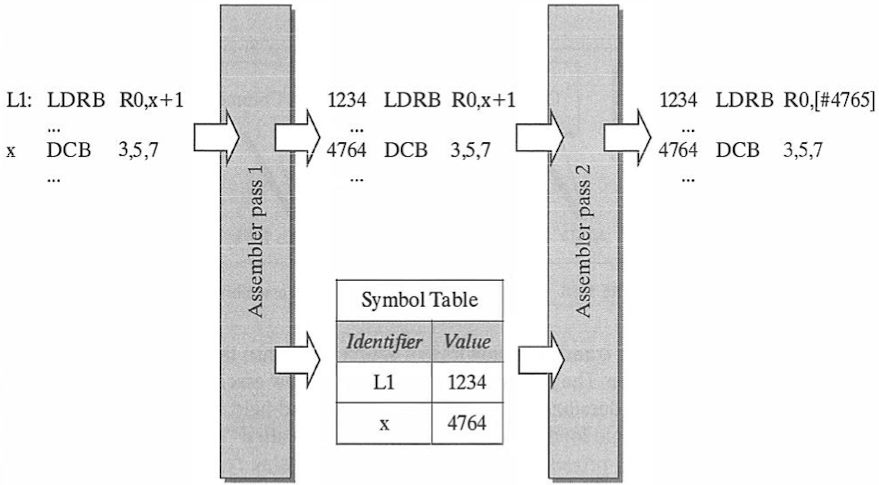
\includegraphics[width=8.5cm]{images/SoftwareDevelopmentProzess}
\end{minipage}

\subsection{Assembly-Language Syntax}
\begin{tabular}{llll}
    \textbf{Lable}  &\textbf{OpCode}  &\textbf{Operand}  & \textbf{Comment} \\ 
    L1  & ADD &R0,R1,\#5    & Replace R0 by sum of R1 and 5 \\ 
    FUNC& MOV &R0,\#100     & this sets R0 to value 100 \\  
        & BX  &LR           & this is a function return\\
\end{tabular} 
\begin{tabular}{|ll}
    \textbf{Lable}  & optional  \\ 
    \textbf{OpCode} & spezifiziert den Befehl \\ 
    \textbf{Operand}& Parameter  \\ 
    \textbf{Comment}&  optionale Beschreibung\\ 
\end{tabular} 
\\
\begin{multicols}{2}
    \begin{minipage}{\linewidth}
        \subsection{Unified Assembler Language (UAL)}
        Syntax für ARM und Thumb Instructionen.\\
        Die meisten Instruktionen arbeiten mit Registern\\
        \textbf{BSP}\newline
        \begin{tabular}{lll}
            MOV&R2,\#100  &;R2=100,Direkte Zuweisung  \\ 
            LDR&R2,[R1]   &;R2= den Wert von R1  \\ 
            ADD&R2,R0     &;R2=R2+R0  \\ 
            ADD&R2,R0,R   &;R2=R0+R1  \\ 
        \end{tabular} 
    \end{minipage}
    
    \begin{minipage}{0.8\linewidth}
        \subsubsection{Register List}
        \begin{tabular}{lll}
            Norm. Form&{reglist}  &;{R1,R2...Rn}  \\ 
            PUSH& {LR} & ;save LR on stack\\ 
            POP&  {LR}&  ;remove from stack; place in LR\\  
            PUSH& {R1-R3,LR} & ;save R1,R2,R3; return address\\  
            POP& {R1-R3,PC} &;restore R1,R2,R3 and return \\ 
        \end{tabular} 
    \end{minipage}
\end{multicols}

\subsection{Addressing}
 \subsubsection{Immediate Adressing}
\begin{minipage}{10cm}
        Der Datenwert ist unmittelbar in der Instruktion erhalten. Daher kein zusätzlicher Speicherzugriff erforderlich\newline
        Form: \# imm\newline
        \colorbox{lightgray}{
        \begin{tabular}{lll}
             MOV & R0,\# 100&;R0=100, immediate addressing \\ 
        \end{tabular} }
\end{minipage}
%
\begin{minipage}{0.5cm}
	\-\
\end{minipage}
%
\begin{minipage}{8cm}
	 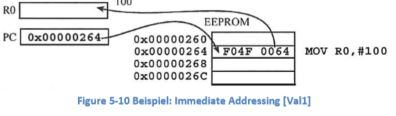
\includegraphics[width=8cm]{images/immediateAddressing}    
\end{minipage}  

\subsubsection{Indirect Addressing}
\begin{minipage}{10cm}
        Bei der \textit{Indirect Addressing} Modes sind die Daten im Memory. Ein Register enth"alt irgendwie einen Zeiger auf diese Daten. Nach der \textit{Fetch}-Phase , bei welcher die Instruktion aus dem Programmspeicher gelesen wird,
        sind noch einer oder mehrere Speicherzugriffe erforderlich um die Daten zu lesen oder zu schreiben.\newline
        Form: [Rn]\newline
        \colorbox{lightgray}{
        \begin{tabular}{lll}
            LDR & R0,[R1]&;R0=value pointed to by R1 \\ 
        \end{tabular} }\\
        \textbf{R1 wird nicht verändert}
\end{minipage}
%
\begin{minipage}{0.5cm}
	\-\
\end{minipage}
%
\begin{minipage}{8cm}
	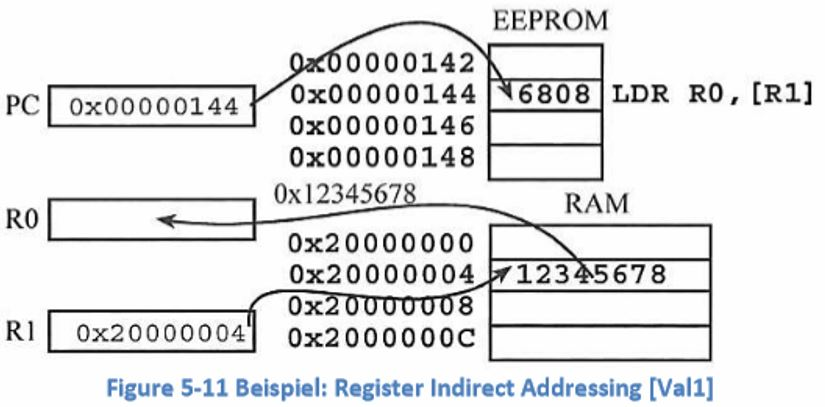
\includegraphics[width=8cm]{images/indirectAddressing}    
\end{minipage}

\subsubsection{Register Addressing with Displacement}
\begin{minipage}[b]{10cm}
        Dasselbe, nur wird hier dem Wert R0 noch \# 4 hinzugefügt\newline
        R1 bleibt weiterhin unverändert.\newline
        Form: [Rn,\# imm]\newline
        \colorbox{lightgray}{
        \begin{tabular}{lll}
            LDR & R0,[R1,\# 4]&;R0=word pointed to by R1+4 \\ 
        \end{tabular} }\\
\end{minipage}
%
\begin{minipage}{0.5cm}
    	\-\
\end{minipage} 
%
\begin{minipage}{8cm}
    	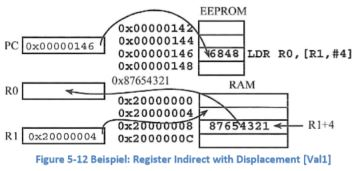
\includegraphics[width=8cm]{images/AddressingDisplacment}    
\end{minipage}

\subsubsection{Register Indirect with Index}
Form: [Rn,Rm]\newline
\colorbox{lightgray}{
\begin{tabular}{lll}
   LDR &R0,[R1,R2]  &;R0= word pointed to by R1+R2 \\ 
\end{tabular} }

\subsubsection{Register Indirect with shifted Index}
Form: [Rn,Rm,LSL \# imm]\newline
\colorbox{lightgray}{
\begin{tabular}{lll}
    LDR&R0,[R1,R2;LSL \#2]  &;R0= word pointed to by R1+4*R2  \\ 
\end{tabular} }

\subsubsection{Register Indirect with Pre-index}
Form: [Rn,\# offset]!\newline
\colorbox{lightgray}{
\begin{tabular}{lll}
   LDR & R0,[R1,\#4]! &;first R1=R1+4, then R0= word pointed to by R1  \\ 
\end{tabular} }

\subsubsection{Register Indirect with Post-index}
Form: [Rn],\# offset\newline
\colorbox{lightgray}{
\begin{tabular}{lll}
    LDR& R0,[R1],\#4  &;R0= word pointed to by R1, then R1=R1+4  \\ 
\end{tabular} }

\subsubsection{PC-relativ}
PC wird als Pointer verwendet.
Form: lable\newline
\begin{tabular}{lll}
    B   &Location   &;jump to Location\\ 
    BL  &Subroutine &;call Subroutine, Rücksprungadresse wird gespeichert\\ 
\end{tabular} 

\subsubsection{Speicher- und I/O-Zugriffe}
\begin{minipage}{10cm}
    Es benötigt immer zwei Instruktionen um auf Daren im RAM oder I/O zuzugreifen.
    $\rightarrow$ PC-Relative Addressierung wird verwendet
    \begin{enumerate}
        \item Erstellt Zeuger auf das Objekt
        \item Greift über den Zeiger Indirekt auf den Speicher zu
    \end{enumerate}
    \colorbox{lightgray}{
    \begin{tabular}{lll}
        LDR   &R1,Count   &;R1 points to variable Count\\ 
        LDR   &R0,[R1]    &;R0= value pointed to by R1\\ 
    \end{tabular} }
\end{minipage}
%
\begin{minipage}{0.5cm}
	\-\
\end{minipage}
%
\begin{minipage}{8cm}
	\includegraphics[width=\linewidth]{images/AddressingRAM}   
\end{minipage}





















